\documentclass[11pt]{article}
\usepackage[a4paper,margin=0.82in]{geometry}
\usepackage{amsmath,amssymb}
\usepackage{booktabs}
\usepackage{graphicx}
\usepackage{microtype}
\usepackage{enumitem}
\usepackage{natbib}
\usepackage{longtable,tabularx,array,multirow}
\usepackage{xcolor}
\usepackage[hidelinks]{hyperref}
\usepackage[nameinlink,noabbrev]{cleveref}
\usepackage{url}

\title{Return-to-Source Hysteresis in Test-Time Adaptation:\\
Configuration Effects, Method Stability, and CIFAR-C External Validation}
\author{Anonymous Authors}
\date{}

\newcommand{\Habs}{\ensuremath{H_{\mathrm{abs}}}}
\newcommand{\Hupd}{\ensuremath{H_{\mathrm{upd}}}}
\newcommand{\Hrel}{\ensuremath{H_{\mathrm{rel}}}}
\newcommand{\A}{\ensuremath{A}}
\newcommand{\B}{\ensuremath{B}}
\newcommand{\C}{\ensuremath{C}}

\begin{document}
\maketitle

\begin{abstract}
Test-time adaptation (TTA) changes a deployed model with unlabeled target batches. A stream can later return to a source-like condition, yet one-way accuracy averages hide the state carried into that return. We define return-to-source hysteresis as the difference between checkpoint source accuracy and clean-return accuracy before return-stage updating. The primary formal campaign contains 1,000 verified CIFAR-10/100 jobs. Four independent expansion campaigns add 60 modern-baseline jobs, 120 normalization-policy jobs, 1,080 trajectory and hyperparameter jobs, and 2,700 CIFAR-10-C/100-C jobs. In the original normalization protocol, four adaptive controls cluster near $H_{\mathrm{abs}}=0.0061$ and $H_{\mathrm{upd}}$ is near zero, while a normalization ablation changes $H_{\mathrm{abs}}$ from 0.0061 with frozen running statistics to 0.0611 when running statistics adapt. Under the fixed-statistics external protocol, aggregate $H_{\mathrm{abs}}$ is 0.0676 for TENT, 0.6491 for EATA, 0.0367 for SAR, 0.0031 for CoTTA, and 0.0001 for RoTTA. These are independent reimplementation results, not a universal leaderboard. The prospective mechanism screen remains negative. The evidence supports a two-part conclusion: normalization policy explains most of the original endpoint, while update-induced loss varies sharply across methods and corruption settings. The completed baseline, normalization, trajectory, and CIFAR-C campaigns support a bounded empirical characterization. Publication sufficiency remains conditional on target-venue verification and author-controlled submission metadata; the fresh manuscript-wide claims audit is PASS.
\end{abstract}

\noindent\textbf{Keywords:} test-time adaptation; recurrent distribution shift; source recovery; continual learning; online inference; reproducibility

\section{Introduction}
\label{sec:intro}

\paragraph{Plain-language context.}
In practical terms, we ask whether a model that adapts while conditions are unusual behaves differently when a familiar condition returns. We measure the first clean return before allowing another update, so the endpoint describes the state brought back by adaptation rather than the benefit of a later recovery step.

Test-time adaptation (TTA) updates a source-trained model after deployment without labels for incoming examples. Entropy minimization can improve predictions on a shifted stream, while the same updates alter the model state that will process later examples \citep{tent,continual,eata}. Recent surveys place these methods within a broader family of test-time robustness and adaptation procedures \citep{survey}. This state dependence matters when operating conditions recur. A camera can return to a previous illumination, a sensor can revisit a calibration range, and a service can move back to a prior domain.

Most TTA evaluations average accuracy along a one-way stream or measure final forgetting after the stream ends. Those summaries do not identify what happens at the instant a source-like condition returns. They also mix two effects: a normalization configuration change that occurs when adaptation starts, and the parameter updates that accumulate during the intervening stages. We isolate the return event with an endpoint that compares the original checkpoint with a clean source-like evaluation before return-stage adaptation.

The paper answers three questions. First, does a recurrent source-like return produce a positive endpoint across datasets, shifts, trajectories, and source seeds? Second, do simple reversible controls change the endpoint at the same update budget? Third, can update statistics measured before the return outcome predict the update-induced component on an untouched source seed? The third question has a strict timing requirement. A statistic computed after the return evaluation cannot serve as a prospective predictor.

The study makes four contributions.
\begin{enumerate}[leftmargin=1.4em]
    \item We define a return-to-source hysteresis estimand, together with a decomposition that separates a configuration gap from the incremental update-induced component.
    \item We provide a frozen 1,000-job matrix on CIFAR-10 and CIFAR-100 with two recurrent trajectories, five shift families, two severities, five methods, and five source-training seeds.
    \item We report matched-stream comparisons for TENT and three diagnostic recovery controls, including target utility, return accuracy, drift, and wall-clock time.
    \item We preserve the unsupported prospective mechanism screen and the formal admission audit, including the earlier invalid campaign, instead of turning a negative diagnostic into a positive explanation.
\end{enumerate}

The evidence supports a bounded descriptive claim. Adaptive configured states in the tested CIFAR regime show a small checkpoint-to-return loss, while the update-induced component remains near zero and the four adaptive methods do not separate on the primary endpoint at five seeds. Source inference removes the loss but gives lower target accuracy. The paper therefore reports a measurement and its boundaries; it does not claim a new method or a general solution to continual TTA.

\section{Related work and positioning}
\label{sec:related}

\paragraph{Unlabeled test-time adaptation.}
TENT adapts batch-normalization affine parameters by minimizing prediction entropy on each target batch \citep{tent}. Test-time training adds an auxiliary self-supervised objective to update a model at inference \citep{ttt}. MEMO uses augmented views of a test example to create an adaptation signal \citep{memo}. These methods motivate measuring the state after online updates, but their primary evaluations focus on target performance under a stream.

\paragraph{Continual and dynamic streams.}
Continual TTA studies a sequence of domains and the resulting source forgetting \citep{continual}. Efficient Test-Time Model Adaptation without Forgetting (EATA) removes unreliable samples and adds a Fisher-weighted regularizer to limit harmful updates \citep{eata}. NOTE addresses temporal correlation in a continual stream \citep{note}, while sharpness-aware adaptation (SAR) stabilizes updates in dynamic settings \citep{sar}. Robust Test-Time Adaptation in Dynamic Scenarios (RoTTA) uses class-balanced memory and teacher updates \citep{rotta}. CoTTA uses teacher restoration and stochastic recovery \citep{continual}. We independently reimplemented EATA, SAR, CoTTA, and RoTTA, bound each to a pinned upstream behavior reference, and evaluated them under a shared fixed-statistics protocol. The comparison remains descriptive because shared hyperparameters do not reproduce every paper-specific training recipe.

\paragraph{Source recovery and order.}
Back to the Source uses a diffusion-driven source-recovery objective \citep{source}. Cyclic TTA studies a task-specific monocular-video cycle \citep{cyclic}. Order-aware TTA makes temporal order an explicit input to the adaptation problem \citep{order}. A return-to-source endpoint complements these settings by fixing the outcome at the first clean return and separating it from any subsequent recovery update. The exact-region closest-work audit found no retrieved work that covers the complete endpoint, decomposition, and recurrent protocol. The positioning claim remains bounded to this estimand and protocol.

\paragraph{Corruption benchmarks and calibration.}
CIFAR-10 and CIFAR-100 provide public image classification benchmarks \citep{cifar}. CIFAR-10-C and CIFAR-100-C organize common corruptions into severity levels for robustness testing \citep{cifarcorrupt}. We use synthetic operators on uncorrupted test images for controlled recurrence and provenance checks, then evaluate the standard CIFAR-10-C and CIFAR-100-C corruption suite at severities 1, 3, and 5. We report expected calibration error as a secondary descriptor following the calibration literature \citep{calibration}.

\section{Research questions and estimands}
\label{sec:estimands}

Let $\A$ denote the source-like distribution. Let $\B$ and $\C$ denote intervening distributions. A source checkpoint first receives a clean evaluation on $\A$. The adaptation loop then consumes unlabeled batches from a registered trajectory, either $\A\to\B\to\A$ or $\A\to\B\to\C\to\A$. We evaluate $\A$ immediately after the intervening stages and before any update using the returning $\A$ batches.

Let $a_0$ be checkpoint accuracy on $\A$, $a_c$ be the configured-method accuracy on $\A$ before the intervening stream, and $a_r$ be the clean-return accuracy before return-stage adaptation. We define
\begin{equation}
    \Habs = a_0-a_r, \qquad
    G = a_0-a_c, \qquad
    \Hupd = a_c-a_r.
\end{equation}
The decomposition $\Habs=G+\Hupd$ holds row by row. $G$ captures the configuration gap introduced when an adaptive method changes batch-normalization behavior before the stream. $\Hupd$ isolates the additional change associated with the intervening updates. Positive $\Habs$ and $\Hupd$ indicate lower accuracy at return.

The relative endpoint is $\Hrel=\Habs/\max(a_0,10^{-8})$. We treat the source-training seed as the independent replication unit because each seed produces a checkpoint shared across all methods, trajectories, shifts, and severities. Rows within a seed provide repeated conditions for estimating a seed-level mean; they do not provide independent samples for a row-level significance test.

The preregistered questions are:
\begin{description}[leftmargin=1.6em,style=nextline]
    \item[RQ1:] Is $\Habs$ positive and stable across the registered datasets and trajectory classes?
    \item[RQ2:] Do the anchor, EMA restoration, or periodic reset controls reduce $\Habs$ relative to TENT under matched batches and update counts?
    \item[RQ3:] Do entropy, gradient norm, update norm, and pre-return parameter drift predict $\Hupd$ on an untouched seed?
\end{description}
RQ3 requires every predictor measurement to occur before the return outcome. The current campaign satisfies that ordering rule, but its single held source seed and weaker predictor fit do not support a mechanism claim.

\section{Methods}
\label{sec:methods}

\subsection{Data, split, and source checkpoints}
\label{sec:data}

 We use the public CIFAR-10 and CIFAR-100 image classification datasets \citep{cifar}. The provenance manifest records the original archive sources, archive checksums, extracted file sizes, and SHA-256 hashes for every file consumed by the campaign. We train a separate CIFAR-adapted ResNet-18 for each dataset and source-training seed. The architecture follows the residual design of \citet{resnet}; the first convolution uses a $3\times3$ kernel with stride one, and we remove the ImageNet max-pooling layer for $32\times32$ images.

We train each source checkpoint for 30 epochs with stochastic gradient descent (SGD), learning rate $0.1$, momentum $0.9$, weight decay $5\times10^{-4}$, and batch size 256 using PyTorch \citep{pytorch}. A seed controls source initialization, data-loader shuffling, and the deterministic transform generators. We retain seeds 0 through 4. The test split supplies the clean $\A$ evaluation and the transformed $\B$ and $\C$ streams; adaptation never receives labels.

\subsection{Recurrent trajectories and shift operators}
\label{sec:shifts}

Each formal job selects one of two trajectories. The $\A\to\B\to\A$ path has one shifted stage and a clean return. The $\A\to\B\to\C\to\A$ path adds a fixed channel permutation at $\C$. The channel permutation remains outside the $\B$ family, so comparisons among $\B$ families hold the second intervening stage constant.

The $\B$ stage applies one of five operators: additive Gaussian noise, brightness shift, contrast reduction, average-pooling blur, or spatial rotation. Severity 1 and severity 2 use the registered transform parameters in the runner. The transform generator combines the job seed with a stage-specific offset, which makes each shard deterministic while preventing accidental reuse of one random stream across stages. Every stage uses the same test examples and the same order for all methods sharing a job identity.

\subsection{Methods and state-transition contracts}
\label{sec:methods-contract}

Source inference is the non-adaptive reference. It holds the model in evaluation mode, performs no optimizer step, and leaves parameters and batch-normalization buffers unchanged. TENT adapts batch-normalization affine parameters with entropy minimization. The implementation disables running-statistics tracking for the adaptive batch-normalization layers, so the configured source evaluation and the checkpoint source evaluation can differ.

The anchor control adds a coefficient $0.05$ times the squared distance from the source affine parameters to the entropy loss. EMA restoration applies the same entropy update and then moves the affine parameters toward the source with decay $0.99$. Periodic reset applies the entropy update and restores the affine parameters to the source every eighth update. These diagnostic controls test state reversibility under a common stream; they do not implement CoTTA, EATA, SAR, or RoTTA.

The method contract declares which state may change. Source inference allows no parameter, buffer, optimizer, or mode mutation. TENT and the controls allow batch-normalization affine parameters to change; they declare the running-statistics policy and the recovery state separately. The semantic canary checks the contract at the state-dictionary, buffer, optimizer-step, parameter-delta, and event-order levels. An unexpected mutation fails admission.

\subsection{Temporal availability and outcome timing}
\label{sec:timing}

For every batch, the runner assigns an event or step identifier. The target-stream accuracy and entropy use detached predictions produced before the current update. The prospective screen records predictor summaries from the intervening stages, then records a return outcome at the next event. The return outcome contains accuracy before return-stage adaptation and accuracy after one additional return-stage pass.

The primary endpoint always uses the pre-update return accuracy $a_r$. The post-update return accuracy is secondary and describes the immediate effect of an additional adaptation pass. The analysis rejects a prospective mechanism claim whenever a predictor aggregates events at or after the outcome event. This rule excludes future information from explanations of already observed endpoints.

\subsection{Formal admission and provenance binding}
\label{sec:admission}

The campaign passed a retrospective formal admission gate before analysis. The semantic canary covered 20 cases: all five methods, both trajectories, two representative seeds, one shift family, and one severity. The canary verified source immutability, the declared mutation set for each adaptive method, temporal ordering, and result identity. The early online audit checked 370 completed shards, including 80 source shards, before the campaign reached completion.

The admission ledger records the frozen identities. Every result shard binds its own result hash to these identities. The table shows the first and last eight hexadecimal characters; the ledger stores the full SHA-256 values.
\begin{center}
\scriptsize
\begin{tabular}{ll}
Runner & \texttt{160e3a76...a5921c96}\\
Supervisor & \texttt{9c0f24c1...956d8c9a}\\
Manifest & \texttt{875cb278...f556cc29}\\
Dataset provenance & \texttt{4a909492...b39f0c9b}\\
Protocol & \texttt{0324b859...1f50bc626}\\
Environment & \texttt{49cbc1d9...ae95988f}
\end{tabular}
\end{center}

We retain the first formal campaign in the archive and exclude it from evidence. Its audit found source batch-normalization contamination, drift timing mislabeling, and incomplete runner-to-dataset provenance. The corrected formal\_v2 campaign preserves the registered variables and corrects the measurement behavior. The provenance audit keeps the frozen runner label and the manifest label visible as a metadata discrepancy; the analysis does not rewrite the raw shards.

\subsection{Statistical analysis}
\label{sec:stats}

We compute method and subgroup means from the 1,000 verified rows. To respect repeated conditions within a seed, we first average all rows belonging to a seed within the requested group and then resample the five seed means. We use 10,000 percentile bootstrap draws with fixed analysis seeds \citep{bootstrap}. The interval describes seed-cluster uncertainty; it does not describe the distribution of future datasets or deployment streams.

For each contrast, we pair seed-level means across the same dataset, trajectory, shift, and severity. The exact two-sided sign-flip test enumerates all $2^5=32$ sign assignments. Holm correction controls the family of three TENT-versus-control contrasts \citep{holm}. We report the raw effect, interval, and corrected $p$ value. Row-level correlations in the mechanism screen remain descriptive because repeated rows share a source seed.

We also report target accuracy on the intervening $\B$ stream, return accuracy before and after the return update, source calibration error, pre-return parameter drift, and wall-clock time. These measures describe utility and state change. They do not create additional confirmatory hypotheses.

\subsection{Publication-grade expansion campaigns}
\label{sec:expansion-methods}

Four independent campaigns extend the primary protocol without modifying its raw shards. The modern-baseline campaign contains 60 CIFAR-10 jobs for Source, TENT, EATA, SAR, CoTTA, and RoTTA across five source seeds and the $A$-$B$-$A$ and $A$-$B$-$C$-$A$ paths. The implementation status for each adaptive method is \texttt{INDEPENDENT\_REIMPLEMENTATION}; EATA, SAR, CoTTA, and RoTTA bind to exact upstream commits recorded in \texttt{configs/modern\_baseline\_upstreams.json}. All methods use the fixed \texttt{bn\_affine\_frozen\_stats} policy so that the endpoint measures update-induced change.

The normalization campaign contains 120 jobs that compare source evaluation, frozen and adaptive batch-normalization statistics, a train/eval policy variant, and independently materialized GroupNorm and LayerNorm checkpoints. GroupNorm and LayerNorm checkpoints are architecture controls because their source-domain accuracy is near chance; they are not pooled with the batch-normalization comparisons. The trajectory campaign contains 1,080 jobs over $A$-$B$-$A$, $A$-$B$-$C$-$A$, $A$-$B$-$A$-$B$-$A$, and $A$-$C$-$B$-$A$, three pass counts, and learning rates $10^{-4}$, $10^{-3}$, and $10^{-2}$, with the same five seeds and six methods.

The external campaign uses the standard CIFAR-10-C and CIFAR-100-C corruption files, 15 corruption types, severities 1, 3, and 5, five seeds, six methods, and the $A$-$B$-$A$ path, for 2,700 jobs. The first campaign stopped after 1,774 valid jobs because an early audit identified one failed RoTTA shard. We preserve that campaign as \texttt{EARLY\_SANITY\_FAIL} and completed the missing 926 cells in \texttt{external\_validation\_cifar\_c\_recovery\_v1} under a new frozen manifest. The combined analysis verifies all 2,700 unique cells while preserving the two campaign identities. All expansion analyses aggregate within source-training seed before inference and report exact sign-flip tests, seed-cluster bootstrap intervals, and registered Holm corrections.

\section{Results}
\label{sec:results}

\subsection{The corrected campaign completed with an auditable matrix}
\label{sec:campaign-result}

The formal\_v2 campaign completed all 1,000 registered jobs with zero current failures. The matrix contains two datasets, five source-training seeds, five methods, two trajectories, five shift families, and two registered severity levels. Each method therefore contributes 200 rows, each dataset contributes 500 rows, and the adaptive subset contributes 800 rows. The analysis loader verified result hashes, checkpoint identities, dataset files, protocol parameters, finite numeric values, and the no-labels-during-adaptation flag before computing any statistic.

Table~\ref{tab:primary} gives the primary endpoint and secondary utility measures. Source inference produces $\Habs=0$ because it preserves the checkpoint state. The adaptive methods cluster between 0.00610 and 0.00637. Their target accuracy clusters around 0.565, whereas source inference averages 0.4796. TENT gains 0.000268 accuracy points on the clean return after the extra return update, but that post-update gain does not remove the checkpoint-to-return gap.

\begin{table}[t]
\centering
\scriptsize
\caption{Primary endpoint, target utility, return accuracy, and pre-return drift. Means use the 200 rows for each method. The primary 95\% intervals use five seed-cluster means and 10,000 bootstrap draws.}
\label{tab:primary}
\begin{tabular}{lrrrrrr}
\toprule
Method & $\Habs$ & 95\% interval & Target acc. & Return pre & Return post & Drift \\
\midrule
Source & 0.000000 & [0, 0] & 0.479609 & 0.733250 & 0.733250 & 0.000000 \\
TENT & 0.006106 & [0.005307, 0.007069] & 0.565139 & 0.727144 & 0.727412 & 0.034742 \\
Anchor & 0.006099 & [0.005308, 0.007056] & 0.565142 & 0.727152 & 0.727400 & 0.034741 \\
EMA restore & 0.006186 & [0.005438, 0.007104] & 0.565055 & 0.727064 & 0.727223 & 0.020432 \\
Periodic reset & 0.006374 & [0.005673, 0.007171] & 0.564559 & 0.726876 & 0.727014 & 0.004280 \\
\bottomrule
\end{tabular}
\end{table}

\begin{figure}[t]
\centering
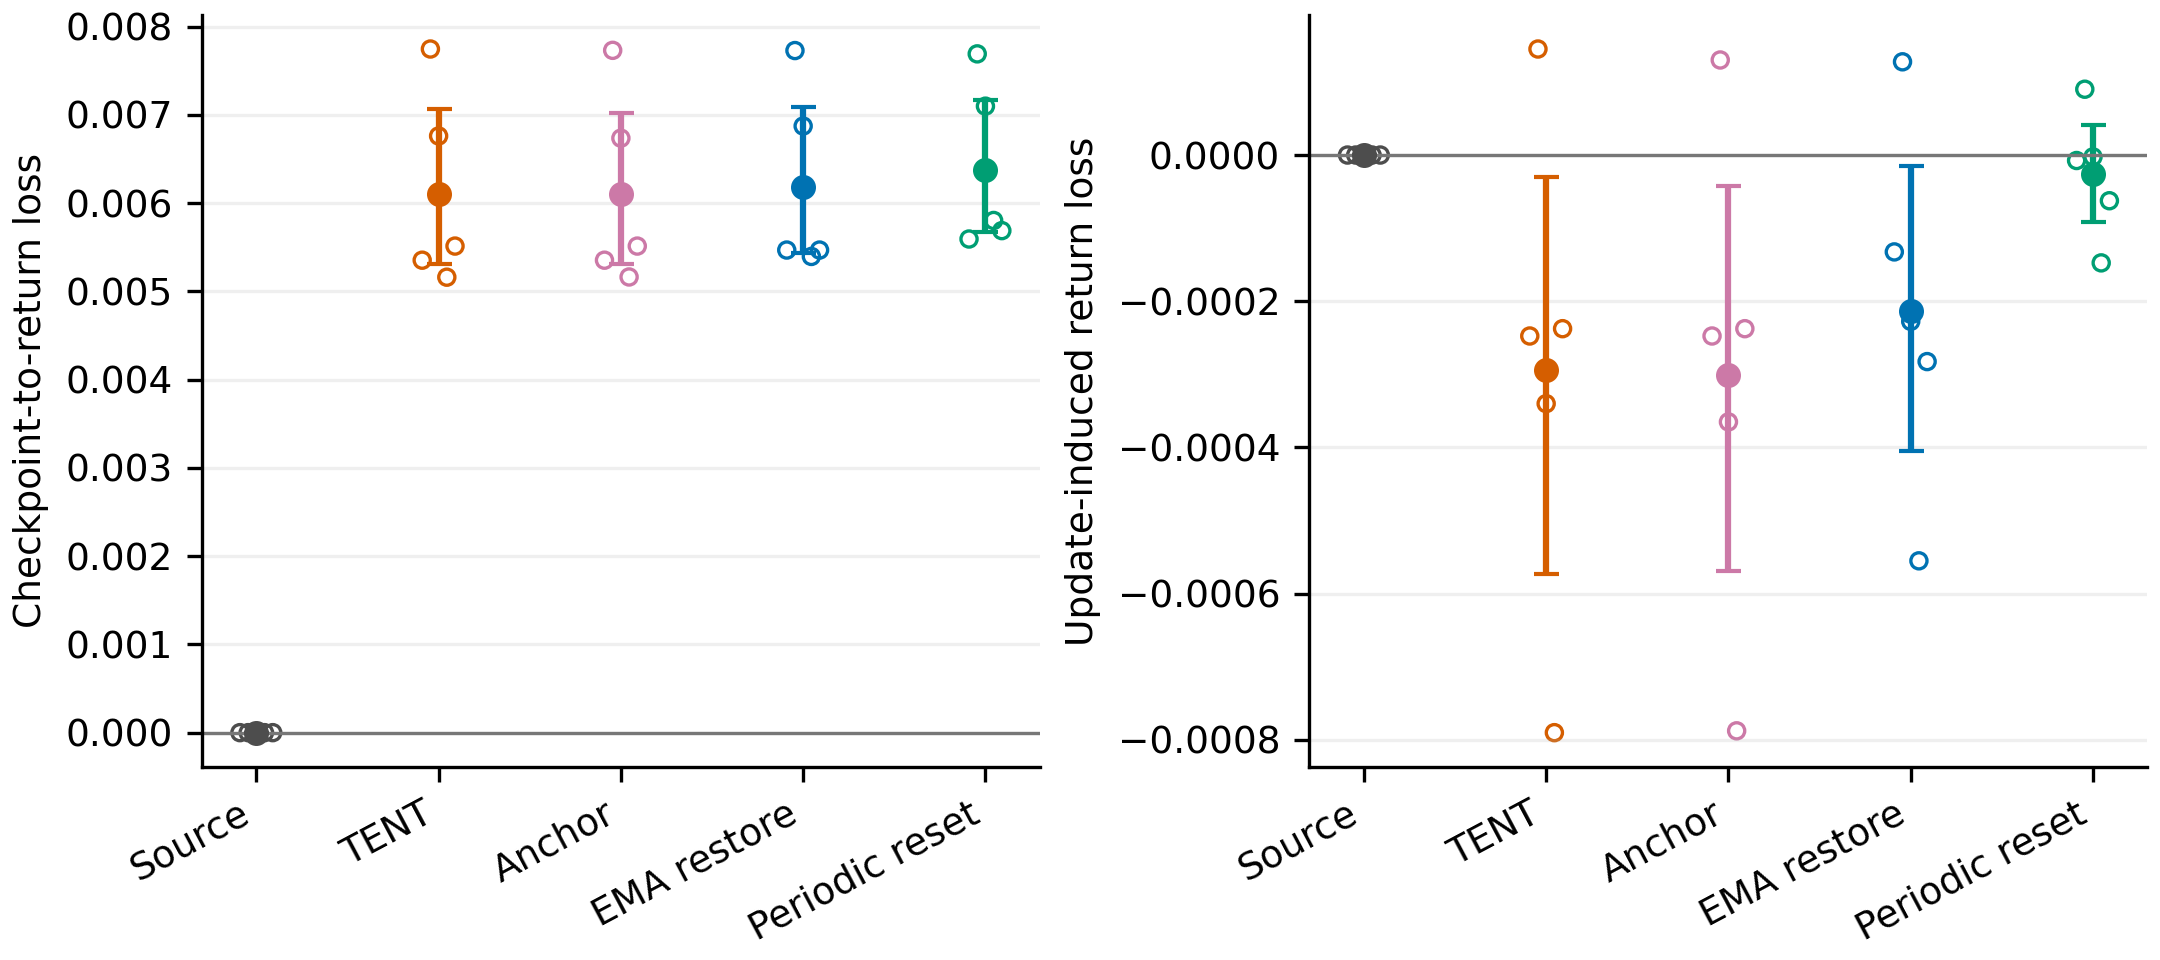
\includegraphics[width=0.94\linewidth]{figures/expansion_return_loss.png}
\caption{Seed-level means and 95\% seed-cluster intervals for checkpoint-to-return loss and update-induced loss. Open points show the five source-training seeds.}
\label{fig:return-loss}
\end{figure}

\paragraph{Takeaway.}
The endpoint is positive for every adaptive seed mean and zero for source inference. The adaptive methods have overlapping intervals, so the matrix does not identify a primary-endpoint winner. The target-accuracy difference between source inference and adaptation is large relative to the differences among adaptive controls.

\subsection{The configuration gap explains most of the endpoint}
\label{sec:decomposition}

The endpoint decomposition separates two state changes.

Adaptive batch-normalization behavior creates one change when adaptation starts. Intervening updates create the second change.
The mean configuration gap $G$ is 0.0064 across adaptive methods after rounding to four decimals. The update-induced means are $-0.000294$ for TENT, $-0.000302$ for the anchor, $-0.000214$ for EMA restoration, and $-0.000026$ for periodic reset. The first three controls show small recovery gains at the pre-update return evaluation. The periodic-reset interval includes zero.

 The source baseline has no configuration gap and no update-induced component. Its source accuracy therefore remains 0.73325 at return. The adaptive methods have a mean pre-return accuracy of 0.7269 to 0.7272. The decomposition attributes most of the measured loss to the initial configuration gap, so a lower total endpoint for one control does not demonstrate source-model improvement from its updates.

\begin{table}[t]
\centering
\scriptsize
\caption{Endpoint decomposition. $G$ is the checkpoint-to-configured-source gap and $\Hupd$ is the configured-source-to-return difference.}
\label{tab:decomposition}
\begin{tabular}{lrrrr}
\toprule
Method & $a_0$ & $a_c$ & $G$ & $\Hupd$ (95\% interval) \\
\midrule
Source & 0.733250 & 0.733250 & 0.000000 & 0.000000 [0, 0] \\
TENT & 0.733250 & 0.726850 & 0.006400 & $-0.000294$ [$-0.000590$, $-0.000031$] \\
Anchor & 0.733250 & 0.726850 & 0.006400 & $-0.000302$ [$-0.000572$, $-0.000045$] \\
EMA restore & 0.733250 & 0.726850 & 0.006400 & $-0.000214$ [$-0.000416$, $-0.000026$] \\
Periodic reset & 0.733250 & 0.726850 & 0.006400 & $-0.000026$ [$-0.000100$, $0.000040$] \\
\bottomrule
\end{tabular}
\end{table}

\paragraph{Takeaway.}
 The configuration gap dominates measured return loss under this implementation. The adaptive update component remains close to zero, and periodic reset has an interval that crosses zero. This decomposition makes the operational endpoint interpretable when adaptive batch-normalization policies differ from the source checkpoint.

\subsection{Dataset and trajectory boundaries}
\label{sec:dataset-boundaries}

 The endpoint varies across datasets. For CIFAR-10, adaptive means range from 0.006524 for the anchor to 0.006575 for periodic reset. For CIFAR-100, they range from 0.005673 for the anchor to 0.006173 for periodic reset. Different class counts and source checkpoints explain the target-accuracy gap; the data do not support a claim that one dataset is intrinsically more hysteretic.

Trajectory length changes the target stream more than it changes the endpoint. The adaptive mean is 0.006253 for $\A\to\B\to\A$ and 0.006130 for $\A\to\B\to\C\to\A$. The longer path produces more pre-return affine drift, with a mean of 0.028757 compared with 0.018340 for the shorter path. That drift difference does not translate into a larger total endpoint in this matrix.

\begin{table}[t]
\centering
\scriptsize
\caption{Adaptive endpoint by dataset and trajectory. Each cell averages the four adaptive methods over 400 rows.}
\label{tab:boundaries}
\begin{tabular}{llrrr}
\toprule
Grouping & Level & $\Habs$ & Target acc. & Pre-return drift \\
\midrule
Dataset & CIFAR-10 & 0.006550 & 0.708807 & 0.011485 \\
Dataset & CIFAR-100 & 0.005832 & 0.421140 & 0.035612 \\
Trajectory & $\A\to\B\to\A$ & 0.006253 & 0.569534 & 0.018340 \\
Trajectory & $\A\to\B\to\C\to\A$ & 0.006130 & 0.560413 & 0.028757 \\
\bottomrule
\end{tabular}
\end{table}

\begin{figure}[t]
\centering
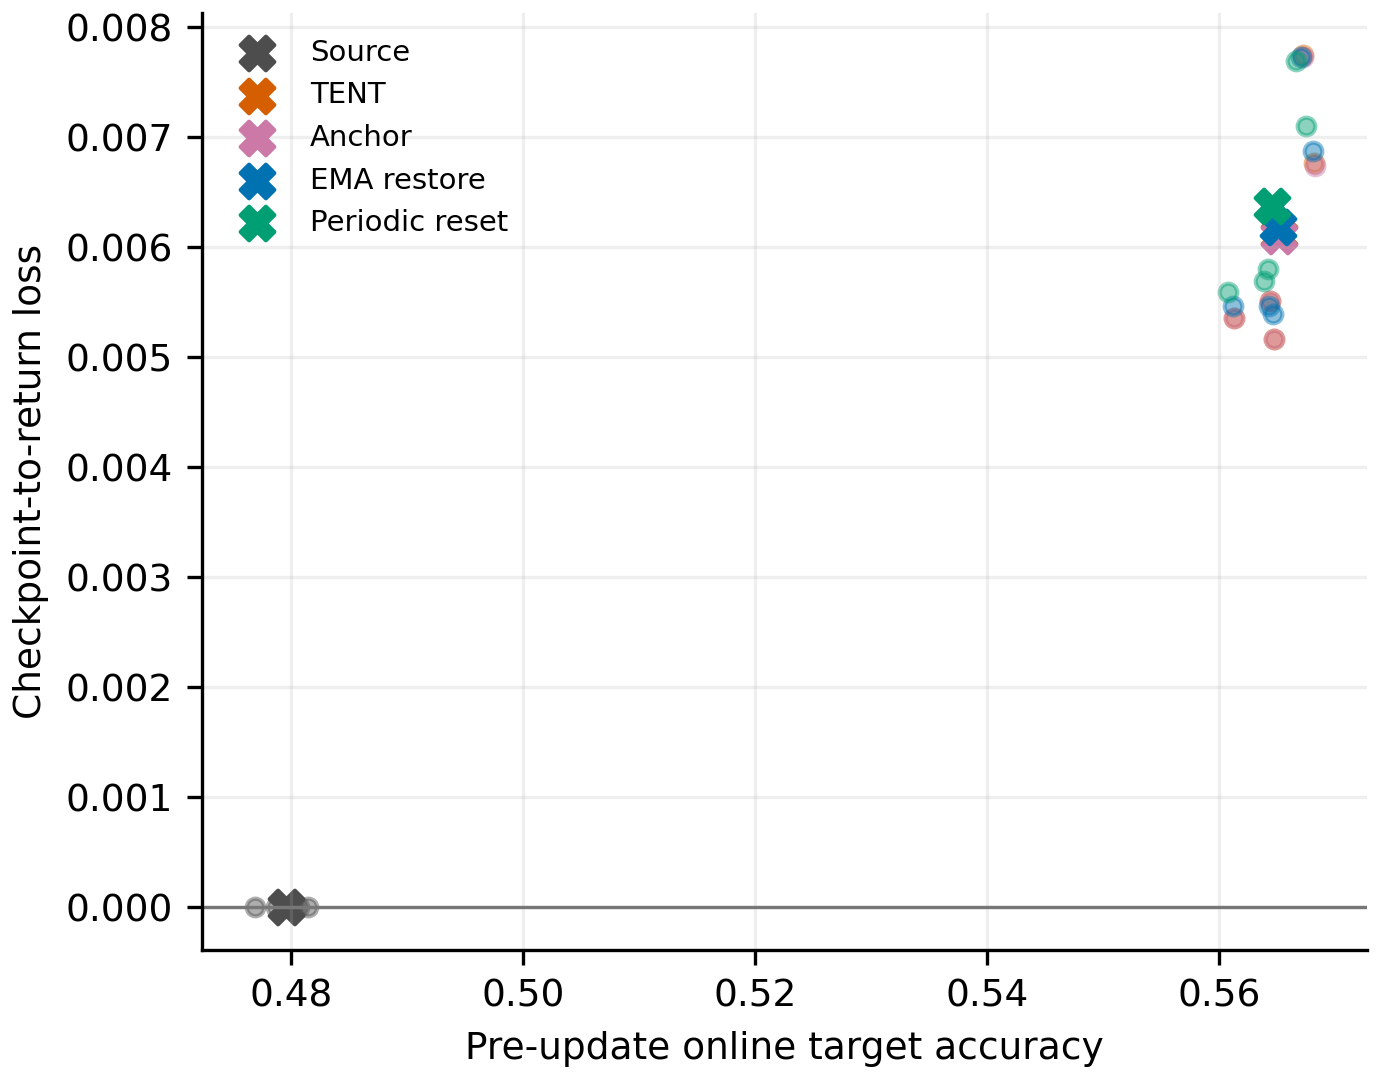
\includegraphics[width=0.92\linewidth]{figures/expansion_target_return_pareto.png}
\caption{Seed-level target utility versus checkpoint-to-return loss. Small points denote seed means; crosses denote method means. Source inference occupies the zero-loss, lower-target-accuracy corner.}
\label{fig:pareto}
\end{figure}

\paragraph{Takeaway.}
The endpoint persists across both datasets and both trajectory lengths, but its magnitude changes with the dataset and control. The longer trajectory increases measured drift while leaving the average endpoint close to the shorter path. These boundaries argue for reporting the full stream design instead of a single aggregate number.

\subsection{Shift and severity boundaries}
\label{sec:shift-boundaries}

The shift-family table reports all five $\B$ operators. Adaptive target accuracy is highest for brightness and contrast, intermediate for blur and noise, and lowest for rotation. The endpoint itself ranges from 0.00608 for blur under the anchor to 0.00638 for periodic reset under noise and contrast. Differences across shift families remain smaller than the configuration gap.

Severity changes target utility while leaving the endpoint nearly unchanged. Adaptive means are 0.006097 at severity 1 and 0.006100 at severity 2 for the anchor, with comparable values for the other controls. The target-accuracy mean falls from 0.5833 to 0.5469 for the anchor as severity increases. This separation shows that source-return loss and target utility capture different operational costs.

\begin{table}[t]
\centering
\scriptsize
\caption{Adaptive results by shift family. Each row averages the four adaptive methods and both trajectories over five seeds and two severities.}
\label{tab:shifts}
\begin{tabular}{lrrr}
\toprule
Shift family & $\Habs$ & Target acc. & $\Hupd$ \\
\midrule
Blur & 0.006182 & 0.578034 & $-0.000218$ \\
Brightness & 0.006198 & 0.676241 & $-0.000202$ \\
Contrast & 0.006243 & 0.675892 & $-0.000157$ \\
Noise & 0.006074 & 0.530596 & $-0.000326$ \\
Rotation & 0.006258 & 0.364105 & $-0.000142$ \\
\midrule
Severity 1 & 0.006192 & 0.583189 & $-0.000208$ \\
Severity 2 & 0.006190 & 0.546758 & $-0.000210$ \\
\bottomrule
\end{tabular}
\end{table}

\begin{figure}[t]
\centering
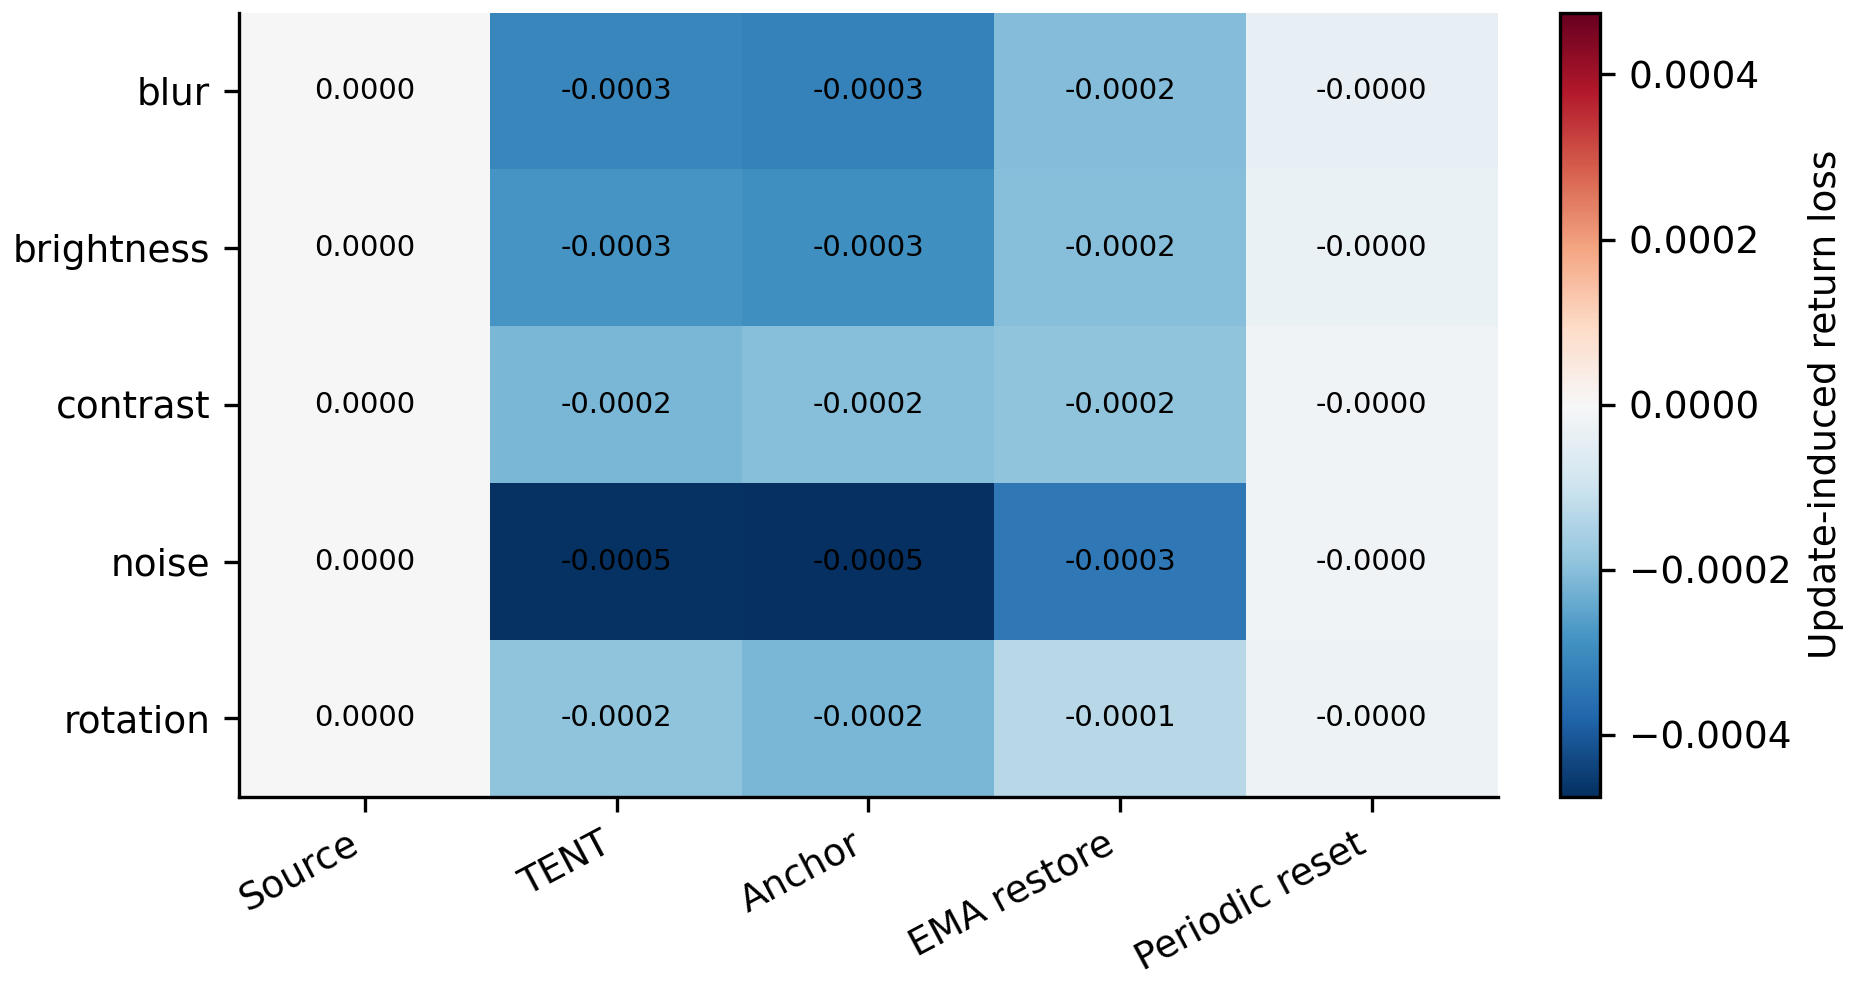
\includegraphics[width=0.93\linewidth]{figures/expansion_shift_method_heatmap.png}
\caption{Mean update-induced component by shift family and method. The signed values stay close to zero relative to the total endpoint.}
\label{fig:heatmap}
\end{figure}

\paragraph{Takeaway.}
The controlled transforms change target accuracy more than they change the return endpoint. The endpoint therefore measures a state-history cost that this protocol partially decouples from severity-dependent target accuracy.

\subsection{Matched controls do not separate at five seeds}
\label{sec:contrasts}

The paired contrasts use the same seed, dataset, trajectory, shift family, and severity for TENT and each control. TENT minus anchor is $0.000007$ for $\Habs$ with Holm-adjusted $p=0.50$. TENT minus EMA restoration is $-0.000080$ with adjusted $p=0.50$. TENT minus periodic reset is $-0.000268$ with adjusted $p=0.375$. The interval for the last contrast is $[-0.000482,-0.000083]$, but the exact sign-flip test does not cross the corrected threshold with five independent seeds.

Target utility contrasts also remain below the corrected threshold. TENT exceeds the periodic-reset target accuracy by 0.000580 with adjusted $p=0.1875$, and its difference from EMA restoration is 0.000084 with adjusted $p=0.1875$. The control table therefore supports a descriptive trade-off: periodic reset has the smallest affine drift and the lowest target accuracy among adaptive methods, while TENT has the largest drift and a nearly identical endpoint.

\begin{table}[t]
\centering
\scriptsize
\caption{Paired TENT-minus-control contrasts. Positive values mean that TENT has the larger value. Each test uses five seed-level paired means and Holm correction across the three controls.}
\label{tab:contrasts}
\begin{tabular}{llrrrr}
\toprule
Endpoint & Control & Mean & 95\% interval & $p$ & $p_{\mathrm{Holm}}$ \\
\midrule
$\Habs$ & Anchor & 0.000007 & [$-0.000001$, 0.000018] & 0.5000 & 0.5000 \\
$\Habs$ & EMA restore & $-0.000080$ & [$-0.000163$, 0.000008] & 0.2500 & 0.5000 \\
$\Habs$ & Periodic reset & $-0.000268$ & [$-0.000482$, $-0.000083$] & 0.1250 & 0.3750 \\
Target acc. & Anchor & $-0.000003$ & [$-0.000010$, 0.000003] & 0.4375 & 0.4375 \\
Target acc. & EMA restore & 0.000084 & [0.000059, 0.000113] & 0.0625 & 0.1875 \\
Target acc. & Periodic reset & 0.000580 & [0.000528, 0.000645] & 0.0625 & 0.1875 \\
\bottomrule
\end{tabular}
\end{table}

\paragraph{Takeaway.}
The registered matrix does not support a winner among the four adaptive methods. The controls expose a drift and target-utility trade-off, but five seeds give low resolution for small endpoint differences. The independent modern-baseline campaign is complete. Its shared-protocol results support descriptive comparison under the stated implementation boundary, not a universal ranking.

\subsection{The prospective mechanism screen fails its held-seed test}
\label{sec:mechanism}

The mechanism screen fits a control model and a predictor model on seeds 0 through 3. The predictor inputs are entropy, gradient norm, update norm, and pre-return affine drift. The training fit has mean absolute error (MAE) 0.000266 and coefficient of determination $R^2=-0.399$ for the predictor model, compared with MAE 0.000258 and $R^2=-0.266$ for the control model. Incremental $R^2$ is $-0.134$, and incremental MAE reduction is $-0.000008$.

 The held screen uses seed 4. It contains 160 held rows that share the same seed, so the screen cannot establish cross-seed generalization. The predictor fit also underperforms the control model, with negative incremental $R^2$ and MAE reduction. We retain the screen and its diagnostic figure, but we withdraw the prospective mechanism claim. We formally abandon the prospective predictor question for this manuscript. A future test on fresh held seeds 5 through 9 would require a new preregistered campaign and would remain separate from the current evidence.

\begin{figure}[t]
\centering
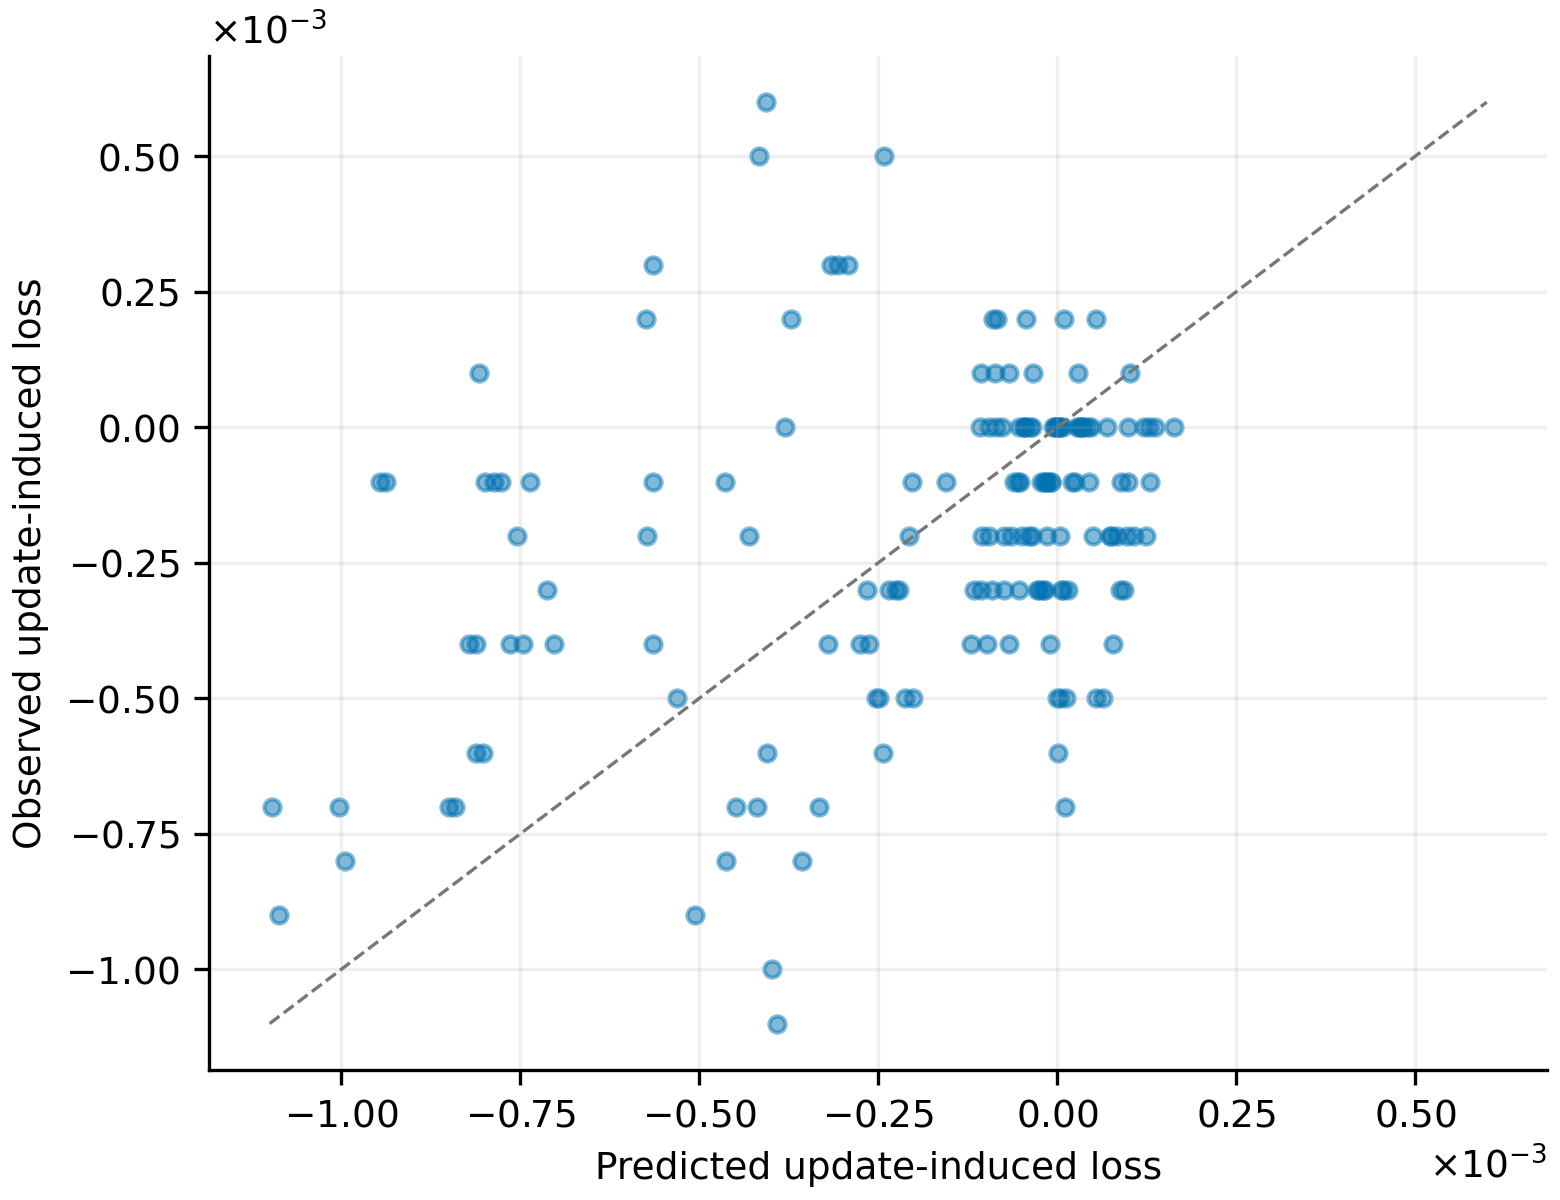
\includegraphics[width=0.88\linewidth]{figures/expansion_mechanism_screen.png}
\caption{Held-seed diagnostic screen. Event ordering passes the pre-outcome availability rule, but one held source seed and a weaker predictor fit prevent a prospective mechanism claim.}
\label{fig:mechanism}
\end{figure}

\paragraph{Takeaway.}
The current data do not identify a predictive mechanism. The negative screen limits the claim to endpoint characterization and documents the held-seed and predictive-performance requirements for a future mechanism campaign.

\subsection{Modern baselines separate under fixed normalization}
\label{sec:modern-baselines}

The 60-job modern-baseline campaign uses the same five source seeds and two recurrent trajectories for Source, TENT, EATA, SAR, CoTTA, and RoTTA. The fixed-statistics policy removes the configuration gap, so $H_{\mathrm{abs}}=H_{\mathrm{upd}}$. Table~\ref{tab:modern} reports seed-level means across both trajectories.

The comparison uses a shared CIFAR protocol. The upstream behavior references remain the semantic anchors, while the local optimizer and threshold settings are recorded in the campaign manifest. The resulting rows are independent reimplementations rather than paper-recipe reproductions.

\begin{table}[t]
\centering\scriptsize
\caption{Protocol differences between pinned upstream references and the shared comparison protocol.}
\label{tab:protocol-differences}
\begin{tabular}{p{0.22\linewidth}p{0.34\linewidth}p{0.34\linewidth}}
\toprule
Component & Pinned reference behavior & Shared campaign protocol\\
\midrule
Model and data & Method-specific upstream settings & CIFAR ResNet-18, fixed source checkpoints, five seeds\\
Normalization & Method-specific normalization policy & BN affine updates with frozen running statistics\\
Sample selection & Method-specific thresholds and filters & Local settings registered per method and shard\\
Optimizer & Upstream optimizer and learning rate & Campaign learning-rate grid and method branch\\
Endpoint & Paper-specific target metric & Clean return before return-stage adaptation\\
\bottomrule
\end{tabular}
\end{table}

\begin{table}[t]
\centering\scriptsize
\caption{Modern baselines under fixed batch-normalization statistics. Intervals use five seed means and 10,000 percentile bootstrap draws.}
\label{tab:modern}
\begin{tabular}{lrrrr}
\toprule
Method & $H_{\mathrm{abs}}$ & 95\% interval & $H_{\mathrm{upd}}$ & Target acc.\\
\midrule
Source & 0.000000 & [0.000000,0.000000] & 0.000000 & 0.636610\\
TENT & 0.005920 & [0.004300,0.007260] & 0.005920 & 0.625405\\
EATA & 0.763290 & [0.759518,0.767060] & 0.763290 & 0.123625\\
SAR & 0.002210 & [0.001470,0.002950] & 0.002210 & 0.638945\\
CoTTA & 0.001610 & [0.000550,0.002780] & 0.001610 & 0.634525\\
RoTTA & 0.000020 & [-0.000030,0.000090] & 0.000020 & 0.636635\\
\bottomrule
\end{tabular}
\end{table}

EATA produces a large loss and low target accuracy in this independent implementation. The result is consistent across five seeds, yet it can reflect sensitivity to thresholding, Fisher selection, optimizer, or checkpoint details. We therefore treat it as an implementation-sensitivity signal. RoTTA has an endpoint interval spanning zero, while CoTTA and SAR remain close to the source state. Exact sign-flip tests with five seeds cannot establish a corrected $p<0.05$ result.

\paragraph{Takeaway.}
Fixed normalization exposes method-specific update behavior that the original formal protocol concealed. The result supports comparative measurement, not a universal ranking.

\subsection{Normalization policy changes the endpoint by an order of magnitude}
\label{sec:normalization-ablation}

The 120-job normalization campaign isolates the evaluation policy on CIFAR-10 noise. Source evaluation and a policy that leaves the source model in evaluation mode produce zero $H_{\mathrm{abs}}$ for Source and TENT. Under frozen batch-normalization running statistics, TENT produces $H_{\mathrm{abs}}=0.006110$ and $H_{\mathrm{upd}}=0.006110$. Allowing running statistics to adapt increases TENT $H_{\mathrm{abs}}$ to 0.061100, while target accuracy rises from 0.622155 to 0.757545. This tenfold change occurs without changing the recurrent path or source checkpoint.

GroupNorm and LayerNorm checkpoints yield source accuracies of 0.100180 and 0.102920. Their $H_{\mathrm{abs}}$ values are 0.000180 and 0.002920, but these checkpoints operate near chance and cannot support a fair architecture comparison. We retain them as exploratory controls.

\paragraph{Takeaway.}
Normalization policy is a load-bearing experimental variable. A return loss measured without reporting running-statistics behavior cannot identify recurrent update damage.

\subsection{Trajectory, recurrence, and hyperparameter expansion}
\label{sec:trajectory-expansion}

The 1,080-job factorial campaign evaluates six methods on four trajectories, three pass counts, and three learning rates. Under its fixed-statistics protocol, TENT has $H_{\mathrm{abs}}=0.311492$, EATA=0.732532, SAR=0.034163, CoTTA=0.010062, and RoTTA=0.000023. The source baseline remains at zero. TENT's $H_{\mathrm{abs}}$ rises by 0.121200 when a single return path becomes recurrent, by 0.055480 from one to two adaptation passes, and by 0.184347 from one to four passes. Its learning-rate contrasts are -0.219752 for $10^{-4}$ versus $10^{-3}$ and 0.493573 for $10^{-2}$ versus $10^{-3}$. These effects are descriptive because five seeds limit exact sign-flip resolution and the campaign uses a different endpoint scale from formal\_v2.

The order-reversal contrast for TENT is -0.019218 for $A$-$C$-$B$-$A$ relative to $A$-$B$-$C$-$A$. CoTTA changes by 0.004493, while RoTTA changes by -0.000002. The direction and magnitude depend on the method, so the data do not support a single order-sensitivity mechanism.

\paragraph{Takeaway.}
Recurrence, pass count, learning rate, and order can dominate the endpoint under fixed statistics, but their effects are method-specific. The expansion bounds the claim to the registered protocol and does not rescue the earlier prospective mechanism model.

\subsection{CIFAR-C external validation reproduces method dependence}
\label{sec:external-validation}

The combined external ledger covers all 2,700 registered CIFAR-C cells. The failed v1 campaign contributes 1,774 valid shards and remains archived with its failed RoTTA job. The recovery campaign contributes the missing 926 shards under a new manifest. The integrity audit finds no missing, duplicated, or extra cell, and every shard passes source immutability and predictor-before-outcome checks.

Under \texttt{bn\_affine\_frozen\_stats}, the configuration gap is zero by construction. The aggregate endpoint is therefore update-induced: $H_{\mathrm{abs}}=H_{\mathrm{upd}}$. Across CIFAR-10-C and CIFAR-100-C, Source has target accuracy 0.565222 and zero loss; TENT has $H_{\mathrm{abs}}=0.067583$ and target accuracy 0.535114; EATA has $H_{\mathrm{abs}}=0.649115$ and target accuracy 0.187878; SAR has $H_{\mathrm{abs}}=0.036729$ and target accuracy 0.550940; CoTTA has $H_{\mathrm{abs}}=0.003145$ and target accuracy 0.562429; RoTTA has $H_{\mathrm{abs}}=0.000117$ and target accuracy 0.565103.

\begin{sloppypar}
The dataset-specific analysis gives the same qualitative boundary with different scales. CIFAR-10-C target accuracies are 0.699199, 0.690510, 0.309556, 0.701484, 0.697594, and 0.698966 for Source, TENT, EATA, SAR, CoTTA, and RoTTA. CIFAR-100-C gives 0.431246, 0.379717, 0.066200, 0.400396, 0.427264, and 0.431240. EATA remains the strongest instability signal, while RoTTA and CoTTA stay close to Source on return.
\end{sloppypar}

\begin{figure}[t]
\centering
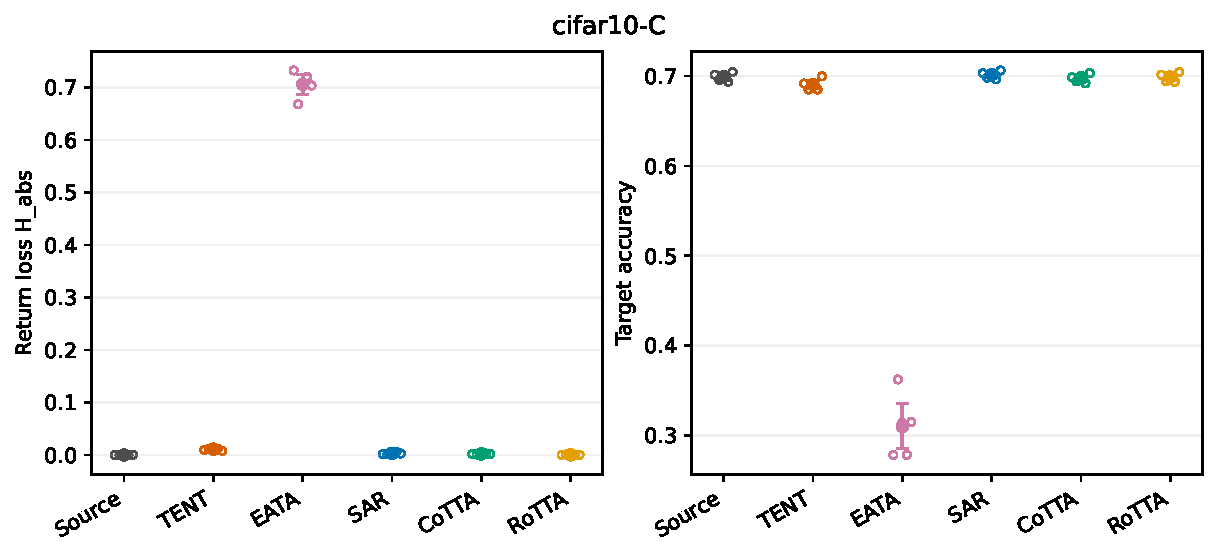
\includegraphics[width=0.95\linewidth]{figures/external_cifar10_c_method_summary.pdf}
\caption{CIFAR-10-C external validation. Points show seed means and intervals show 95\% seed-cluster bootstrap intervals.}
\label{fig:external-cifar10}
\end{figure}

\begin{figure}[t]
\centering
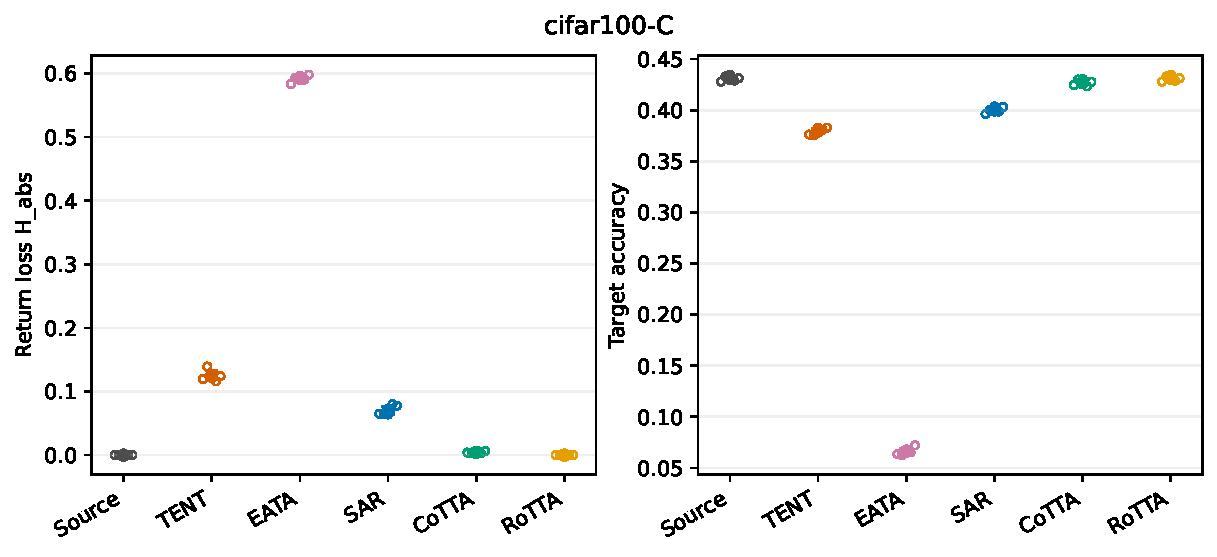
\includegraphics[width=0.95\linewidth]{figures/external_cifar100_c_method_summary.pdf}
\caption{CIFAR-100-C external validation. The method ordering changes in scale but preserves the EATA instability signal.}
\label{fig:external-cifar100}
\end{figure}

\paragraph{Takeaway.}
External standard corruptions reproduce the protocol boundary: fixed normalization reveals update-induced loss, and the loss varies sharply by method and dataset. These results strengthen the measurement claim while ruling out a universal method ordering.

\section{Discussion}
\label{sec:discussion}

The main result is a protocol boundary. In formal\_v2, adaptive CIFAR models return to the clean source distribution with a mean accuracy difference near 0.006, and the update-induced term stays near zero. The normalization ablation changes the endpoint from 0.0061 with frozen statistics to 0.0611 with running-statistics adaptation. This tenfold change identifies normalization policy as a load-bearing part of the estimand.

The method comparison answers a narrower question than a leaderboard. Under fixed statistics, CoTTA and RoTTA stay close to Source on the endpoint, SAR has a small loss, TENT has a larger loss, and EATA becomes unstable. The same ordering appears in standard CIFAR-C aggregates, with dataset-dependent scale. These are independent reimplementation results tied to pinned upstream references, so the paper treats them as protocol-specific evidence and does not generalize them to universal algorithm rankings.

The decomposition clarifies the endpoint. A method can show a positive checkpoint-to-return loss while its intervening updates slightly improve the configured source accuracy. Reporting $H_{\mathrm{upd}}$ alongside $G$ distinguishes a source-normalization policy from recurrent update damage. The external fixed-statistics campaign removes $G$ by construction and therefore measures a different, explicitly update-induced endpoint.

The failed mechanism screen remains part of the scientific result. Its predictor events satisfy the pre-outcome availability rule, but the held set contains one source seed and the predictor model underperforms the control model. The expansion campaigns reveal method-specific trajectory effects, yet they do not validate the proposed predictor. We retain the failure, raw diagnostic artifacts, and the withdrawn mechanism claim.

\section{Limitations and threats to validity}
\label{sec:threats}

The experiment uses CIFAR-10, CIFAR-100, CIFAR-10-C, CIFAR-100-C, one ResNet-18 family, five source-training seeds, synthetic image operators, and one channel-permutation construction for $\C$. These choices give control over recurrence and provenance. They do not establish behavior on natural deployment streams, video, multimodal inputs, or other architectures.

The expansion includes independent CoTTA, EATA, SAR, and RoTTA implementations, normalization controls, and trajectory and hyperparameter ablations. The EATA audit documents protocol differences from the pinned reference, so its extreme endpoint remains an implementation-sensitivity signal rather than a universal method conclusion. The held mechanism screen is a formally closed negative result. The exact-region closest-work audit bounds the positioning claim to the retrieved literature and this protocol. The study still uses one model family and a synthetic corruption benchmark.

The source checkpoints use 30 epochs and a fixed optimizer schedule. Different training budgets, architectures, or normalization layers can change the endpoint. Five seeds give limited resolution for small paired contrasts: the smallest two-sided exact sign-flip $p$ value is 0.0625 before multiplicity correction. We record hardware and package versions, yet deterministic floating-point differences can remain across devices.

\section{Reproducibility and integrity record}
\label{sec:repro}

The project retains the formal manifest, dataset provenance file, source checkpoints, 1,000 formal\_v2 shards, 60 modern-baseline shards, 120 normalization shards, 1,080 trajectory shards, 2,700 external shards, status ledgers, analysis CSV and JSON files, figure triplets, artifact manifests, environment snapshots, admission ledgers, and archived failures. The analysis artifacts record script hashes and bootstrap seeds. Raw shards remain immutable.

The local checks are:
\begin{verbatim}
python -m pytest -q tests/test_formal_campaign_admission.py
python -m pytest -q tests/test_analyze_expansion_results.py
python analyze_expansion_results.py --draws 10000 --force
python -m pytest -q tests/test_external_validation_analysis.py
python external_validation_analysis.py --force
python analyze_modern_baselines.py
python analyze_publication_normalization.py --force
python analyze_publication_trajectory.py --force
\end{verbatim}
The analysis environment records Python 3.13.0, PyTorch 2.9.1, NumPy 2.3.5, pandas 2.3.3, and a CUDA-capable Windows 11 host. The formal\_v2 ledger records four workers, 1,000 completed jobs, zero current failures, and \texttt{restart\_required=false}. The external combined integrity audit records 2,700 unique cells, split between the preserved failed v1 campaign and the completed recovery campaign.

\section{Publication sufficiency and required expansion}
\label{sec:sufficiency}

The manuscript passes the current structural, provenance, numerical-consistency, and advisory-review checks for the expanded CIFAR evidence. Publication sufficiency remains \textbf{FAIL} because the target-venue profile still needs live confirmation and final author metadata, exclusivity, and licensing choices remain author-controlled. The fresh claims audit is \textbf{PASS}. The EATA implementation audit, precision rationale, formal mechanism closure, modern-baseline expansion, normalization ablation, trajectory expansion, exact-region closest-work audit, and standard CIFAR-C validation are complete. Natural deployment shifts and additional architectures remain outside scope.

The current result set supports a bounded technical paper about a protocol-dependent endpoint. It does not support a universal method ranking, a control-superiority claim, or a prospective mechanism explanation. The preserved formal\_v2 and external failure histories remain part of the integrity record. Any reviewer-required experiment must receive a new campaign identity and pass semantic admission before scale-out.

\section{Conclusion}
\label{sec:conclusion}

We define return-to-source hysteresis as a clean-return endpoint that separates checkpoint state, adaptive configuration, and intervening updates. The formal\_v2 campaign shows a small endpoint dominated by normalization configuration. Fixed-statistics modern-baseline and CIFAR-C campaigns reveal method-specific update-induced loss, including an EATA instability signal that requires implementation-sensitive interpretation. The prospective mechanism screen remains negative. The evidence supports a reproducible, protocol-bounded characterization and leaves publication readiness conditional on venue preflight and author-controlled submission checks; the fresh claims audit is PASS.

\section*{Data and code availability}
The public code and derived-artifact archive is available at \href{https://github.com/KaiserIIII/return-to-source-hysteresis}{GitHub repository}. It contains source code, locked environments, manifests, derived analysis tables, figures, and anonymous review materials. Raw CIFAR/CIFAR-C data, checkpoints, per-job shards, logs, and author-only submission files are excluded; the provenance manifests record how to obtain and verify the public datasets. The local archive additionally retains the immutable formal ledgers and raw integrity records.

\section*{Statements and declarations}
\paragraph{Funding.} The author received no specific grant from a public, commercial, or nonprofit funding agency.

\paragraph{Competing interests.} The author declares no competing interests.

\paragraph{Ethics.} This computational study uses public benchmark data and synthetic transforms. It involves no human participants, interventions, or individual-level personal data.

\paragraph{Author contributions.} The authors contributed to conceptualization, methodology, software, formal analysis, investigation, visualization, writing, and project administration.

\paragraph{Use of artificial intelligence.} An AI assistant supported local code orchestration, manuscript drafting, and copy editing. The author inspected the protocol, source outputs, analysis, manuscript, and final PDF and remains responsible for every claim and artifact. The AI assistant is not an author.

\paragraph{Data and code availability.} See the dedicated availability statement above. The author remains responsible for confirming the repository contents, dataset terms, and the final venue-specific data and code statement before submission.

\bibliographystyle{plainnat}
\bibliography{references}

\appendix
\section{Full protocol matrix}
\label{app:matrix}

The formal matrix is the Cartesian product of two datasets, five source-training seeds, five methods, two trajectories, five shift families, and two severities:
\[
2\times5\times5\times2\times5\times2=1{,}000\text{ jobs}.
\]
Each job uses batch size 128, one adaptation pass through each intervening stage, and learning rate 0.001. The source checkpoint training uses 30 epochs, batch size 256, SGD learning rate 0.1, momentum 0.9, and weight decay $5\times10^{-4}$. The source baseline remains in evaluation mode throughout the stream. Adaptive methods update only the declared batch-normalization affine parameters.

\begin{longtable}{p{0.22\linewidth}p{0.68\linewidth}}
\caption{State-transition and evidence contracts.}\label{tab:contracts}\\
\toprule
Contract & Required behavior and checker \\
\midrule
\endfirsthead
\toprule
Contract & Required behavior and checker \\
\midrule
\endhead
Source immutability & Source state dictionary hash, batch-normalization buffers, optimizer step count, trainable-parameter delta, and evaluation mode remain unchanged. \\
Adaptive mutation & TENT and controls change only declared affine parameters; EMA and reset states follow their registered policies. \\
Temporal availability & Predictor event ID precedes outcome event ID. Labels score detached predictions after they leave the adaptation loss. \\
Provenance binding & Runner, supervisor, manifest, dataset, checkpoint, protocol, environment, and result hashes match the frozen ledger. \\
Canary coverage & All methods, both trajectories, two seeds, one representative shift, and one severity pass the semantic checks before scale-out. \\
Early sanity & The supervisor checks source shards, metric ranges, event ordering, hashes, and state mutations during the first 370 completed shards. \\
\bottomrule
\end{longtable}

\section{Admission and failure history}
\label{app:admission}

The admission ledger records a retrospective pass. It reports source immutability PASS, method state-transition PASS, semantic canary PASS, early sanity audit PASS, and \texttt{restart\_required=false}. The first formal campaign remains labeled \texttt{INVALID\_FOR\_PRIMARY\_EVIDENCE} and contributes no row to the analysis. Its three recorded causes are source batch-normalization contamination, drift timing mislabeling, and incomplete runner-to-dataset provenance.

\begingroup\sloppy
\paragraph{Historical campaign accounting.} The exploratory digits pilot contains 10 rows and remains a pilot artifact; it contributes no current claim. We exclude the immutable 960-job protocol-mismatch archive because its stage-pass implementation did not match the frozen protocol. The corrected 960-job digits campaign honored the corrected stage-pass contract, but it uses a separate digits model and transform protocol; its predictor summaries also aggregate post-return updates. We retain it as historical pilot-scale evidence and do not pool it with the CIFAR analysis. The first CIFAR expansion archive contains 1,000 outputs, but the integrity audit marked it \texttt{SUPERSEDED\_INVALID\_FOR\_CLAIMS} after detecting source BatchNorm contamination, post-return drift timing, and missing runner-to-dataset provenance. The current analysis reads only the corrected CIFAR expansion; none of these historical rows enter the primary analysis CSV.
\endgroup

\section{Artifact map}
\label{app:artifacts}
The source is \texttt{paper/main.tex}; the prose copy is \texttt{paper/manuscript.md}.

The primary CSV and JSON files reside in the expansion and publication-expansion analysis directories. The analysis scripts generate PNG, SVG, and PDF figures. The admission ledger resides under \texttt{run\_state/}. The publication sufficiency decision remains a gate and does not imply acceptance by any venue.

\end{document}






